\chapter{Theoretical Background}
\label{chap:terms}
 \section {Forced Alignment and Timing} 
One of the central algorithm  of the modern ASRs is token passing
algorithm. Recognition is the process of producing hypotheses, that fit best
with the audio input. During decoding these hypotheses are
saved as a list of tokens, which contains information about alignment, states
and transitions. \parencite {Young89Token}.

\begin{figure}[htbp]
  \centering
   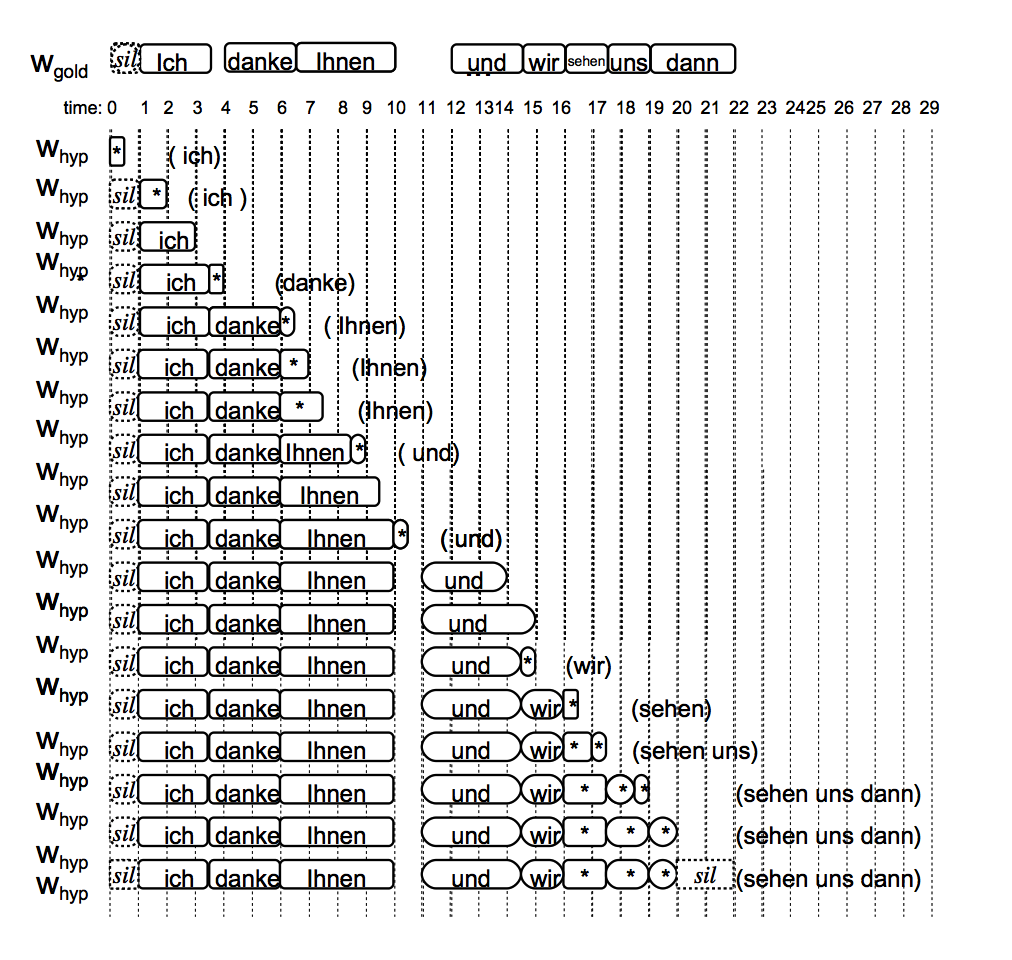
\includegraphics[width=0.9\textwidth]{images/sphinxfa_output.png}
  \caption{incremental output of Sphinx ASR, running in the forced-alignment
  mode}
  \label{fig:sphinxfa}
\end{figure}

Generally, \textit {forced-alignment} is the process of finding the
correspondence between a piece of text and audio speech segments. In the case,
when the transcription is known \textit {forced-alignment} consists only in
determining where in time these particular words occur in the speech segment. 
For example, if we take transcription ``ich danke Ihnen und wir sehen uns dann''
and run Sphinx ASR in the forced-alignment mode with the corresponding audio input than we 
get the following incremental output (see \ref {fig:sphinx}).
By giving the transcription to the recogniser we narrow its search space for hypotheses to
one particular path. Even the recognizer receives some text, that differs from
the ``gold standard'' text, pronounced in our audio, it will still try to align it
to the audio as good as possible. 

By contrast during normal recognition we are dealing with numerous paths  and
possible states in the search graph. During decoding alignment
is computed synchronously together with search states. Final path can differ
from ``gold standard'' transcription, depending on the recognition quality. The
more further recognizer in their hypotheses from the original transcription the
worse recognition quality. Comparison between two sphinx outputs
(see pictures \ref {fig:sphinx} and \ref {fig:sphinxfa}) makes it obvious that
alignment quality depends on recognition quality.
\begin{figure}[htbp]  
  \centering
   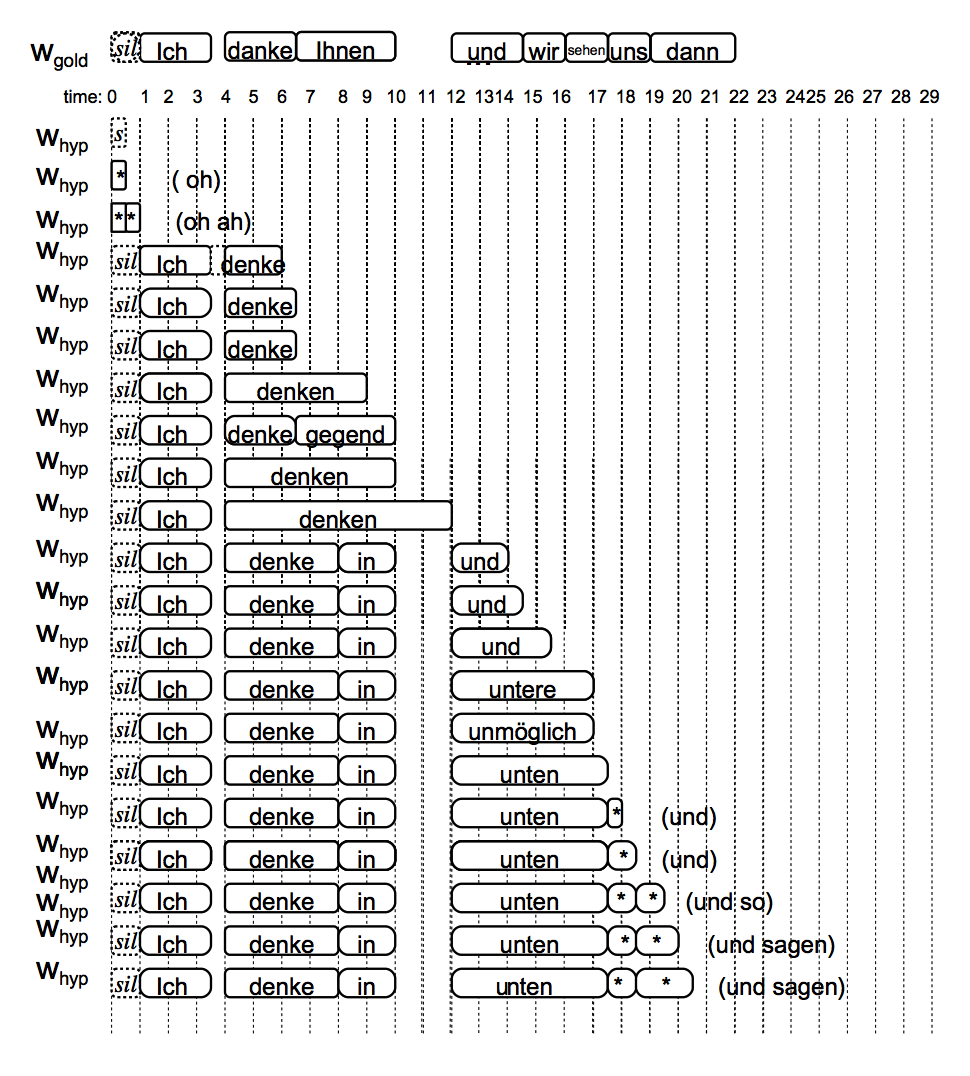
\includegraphics[width=0.9\textwidth]{images/sphinx_output.png}
  \caption{incremental output of Sphinx ASR, running in normal recognition}
  \label{fig:sphinx}
\end{figure}

Forced-alignment is of great importance in fast-moving environments, where
additional non-verbal information, for example gestures, are used.  Without
timing information in such kind of applications it not always possible to
analyse correctly which object is referenced 
\parencite {Baumann2016}.  In contrast to Sphinx, being, a black box, online
Google does not output alignment timing, which makes it impossible to use this 
recognizer for applications, using non-verbal information and context-dependent
object referencing. 

\section {Timeliness in Speech Recognition} 
Timeliness is the second term that is used to characterize word
occurrences during recognition in relation to the time axis. 
To describe the term timeliness the following evaluation metrics are used:
\begin{itemize}
  \item First Occurrence (FO) - is the time between the (true) beginning of a
  word and the first time it occurs in the output (regardless if it is afterwards changed).
\item Final Decision (FD) - is the time between the (true) end of a word and the
time when the recognizer decides on the word, without later revising it anymore.
\end{itemize}

Timeliness is only measured for the words that are correctly recognized or
at least appear in the final output of the recognizer  (\parencite
{Baumann2016}).

In the above depicted output of Sphinx ASR  (see pictures \ref {fig:sphinxfa}
and \ref {fig:sphinx}) FO as well as FD of the word ``ich''  in the first case (forced-alignment mode)
takes plays a half of the slot earlier than in the second case (normal
recognition) and before the word ``ich'' ends in audio. 





 

 